\documentclass[a4paper,12pt]{article}
\usepackage[utf8]{inputenc}
\usepackage{graphicx}
\usepackage{hyperref}
\usepackage{amsmath}
\usepackage{listings}
\lstdefinelanguage{yaml}{
  morekeywords={true,false,null},
  sensitive=false,
  morecomment=[l]{\#},
  morestring=[b]",
  morestring=[b]'
}
\usepackage{color}
\usepackage{geometry}
\geometry{margin=2.5cm}

\title{Activity 1 Report: MQTT Communication with ESP32 and Server}
\author{Eric Muthomi, Pol Vidal}
\date{\today}

\begin{document}

\maketitle

\section{Introduction}
The Internet of Things (IoT) is revolutionizing the way devices communicate and interact. Among the many protocols used in this ecosystem, MQTT (Message Queuing Telemetry Transport) stands out due to its lightweight nature and efficiency. In this activity, we explore the implementation of MQTT communication between an ESP32 development board and an MQTT broker, using Mosquitto as the broker running in a Docker container.

\section{Objectives}
\begin{itemize}
    \item Understand and implement MQTT communication using ESP32.
    \item Use Docker to deploy the Mosquitto MQTT broker.
    \item Collect temperature and humidity data from a DHT11 sensor and publish it to an MQTT topic.
    \item Visualize the real-time data using a subscriber application.
\end{itemize}

% -- Begin new Guiding Questions section with rewritten answers --
\section{Guiding Questions}

\subsection*{Why is MQTT suitable for IoT applications?}
MQTT (Message Queuing Telemetry Transport) is highly suitable for IoT applications because it is a lightweight messaging protocol designed for constrained devices and low-bandwidth, high-latency networks. Its minimal header size of only 2 bytes makes it extremely efficient for microcontrollers such as the ESP32, especially when compared to heavier protocols like HTTP. MQTT also minimizes energy consumption, which is a critical feature for battery-operated IoT devices. Its reliability in adverse network conditions is ensured through multiple Quality of Service (QoS) levels, and its publish-subscribe architecture allows for decoupling of sender and receiver, enhancing scalability and modularity. Originally developed for remote monitoring in harsh environments such as oil pipelines, MQTT remains a robust and versatile choice for modern IoT deployments, including weather stations, smart homes, and industrial monitoring systems.

\subsection*{How does the publish-subscribe model improve efficiency over a request-response model?}
The publish-subscribe model improves communication efficiency by eliminating the need for tight coupling between data producers and consumers. In MQTT, sensors can publish data to a topic without knowledge of who will receive it, while subscribers can receive data without knowing the publisher. This design simplifies system architecture and enables asynchronous communication, which avoids the constant polling required in traditional request-response models like HTTP. Moreover, a single published message can be distributed to multiple subscribers, making it ideal for applications that need to deliver real-time data to multiple endpoints, such as visualization dashboards, databases, or alert systems. This model significantly reduces network overhead, improves scalability, and conserves resources—an ideal setup for bandwidth-constrained and energy-sensitive IoT environments.

\subsection*{What are the advantages of running Mosquitto in a Docker container?}
Running Mosquitto in a Docker container provides portability, reproducibility, and simplified management. Docker ensures that the broker runs in a consistent environment across development and production systems, eliminating platform-specific issues. The setup is streamlined by using official Mosquitto Docker images and configuration files that can be version-controlled. Docker containers also isolate the broker from the host system, enhancing security and reducing dependency conflicts. One notable advantage is the ability to quickly start, stop, or redeploy the broker using Docker Compose, which simplifies orchestration of configurations, persistent data, and logs. When paired with Mosquitto’s lightweight nature, Docker enables a clean, modular deployment that is easy to maintain, scale, and secure.
% -- End new Guiding Questions section with rewritten answers --

% --- Begin updated Methodology and Development section ---
\section{Methodology and Development}

The project implementation consists of three main components: the ESP32 firmware, a Dockerized Mosquitto MQTT broker, and a Python-based real-time visualization subscriber. These components work together to enable data collection, transmission, and monitoring.

\subsection*{System Workflow}

1. ESP32 reads sensor data and publishes it via MQTT. \\
2. Mosquitto broker (in Docker) receives and manages topic subscriptions.\\
3. Python subscriber reads from the topic and plots real-time data.\\

\noindent This modular design promotes clarity, maintainability, and ease of scaling or substitution of components.

\subsection*{ESP32 Firmware}

We developed a C++ script for the ESP32 using the Arduino IDE. This script captures temperature and humidity values from a DHT11 sensor and publishes them to an MQTT topic. The ESP32 connects to a Wi-Fi network and communicates with the Mosquitto MQTT broker running on a server. 

\noindent The following libraries are essential for the firmware:
\begin{itemize}
    \item \texttt{WiFi.h} – manages Wi-Fi connectivity.
    \item \texttt{DHT.h} – interfaces with the DHT11 sensor.
    \item \texttt{PubSubClient.h} – handles MQTT client functions such as connecting, publishing, and maintaining the connection.
\end{itemize}

\noindent A key part of the ESP32 script is the reconnection routine that ensures persistent communication with the MQTT broker. The following code snippet demonstrates how the device attempts to reconnect in case of disconnection:
\begin{lstlisting}[language=C++,caption=MQTT Reconnection Routine]
void reconnect() {
  while (!client.connected()) {
    Serial.print("Connecting to MQTT...");
    if (client.connect("ESP32Client", mqtt_user, mqtt_pass)) {
      Serial.println("connected");
    } else {
      Serial.print("failed, rc=");
      Serial.print(client.state());
      delay(5000);
    }
}
\end{lstlisting}

\noindent This logic ensures the ESP32 stays connected to the broker using user/password credentials. The Mosquitto broker uses a password file (\texttt{pwfile}) where the password is stored in a hashed format, enhancing security.

\newpage
\subsection*{MQTT Broker with Docker}

The Mosquitto MQTT broker is deployed using Docker Compose. This allows for consistent and isolated execution, with persistent configuration, data, and log volumes.

\begin{lstlisting}[language=yaml,caption=Docker Compose File]
version: "3.7"
services:
  mosquitto:
    image: eclipse-mosquitto
    container_name: mqtt-auth
    ports:
      - "1883:1883"
    volumes:
      - ./config:/mosquitto/config
      - ./data:/mosquitto/data
      - ./log:/mosquitto/log
    restart: unless-stopped
\end{lstlisting}


\noindent The Mosquitto configuration includes authentication by specifying a password file:

\begin{lstlisting}[language=,caption=mosquitto.conf]
allow_anonymous false
password_file /mosquitto/config/pwfile
\end{lstlisting}

\noindent To start the broker, the following command is used:
\begin{verbatim}
docker-compose up -d
\end{verbatim}

\subsection*{Python Live Data Subscriber}

The MQTT client is configured with authentication and callback functions to handle connection and message receipt. It starts the loop in the background for continuous message handling.

\begin{lstlisting}[language=Python,caption=MQTT Client Setup]
# MQTT setup
client = mqtt_client.Client()
client.username_pw_set(username, password)
client.on_connect = on_connect
client.on_message = on_message
client.connect(broker, port)
client.loop_start()
\end{lstlisting}

\newpage
\noindent During execution, the script displays a live plot of the incoming temperature and humidity data. Once the user presses Ctrl+C (keyboard interrupt), the script saves a final summary plot showing all recorded data over time.

\begin{lstlisting}[language=Python,caption=MQTT on\_message Callback]
def on_message(client, userdata, msg):
    data = json.loads(msg.payload.decode())
    temps.append(data["temperature"])
    hums.append(data["humidity"])
    timestamps.append(time.time() - start_time)
\end{lstlisting}

To run the subscriber:

\begin{verbatim}
python3 mqtt/liveplot.py
\end{verbatim}

% --- End updated Methodology and Development section ---

% --- Begin Results section with updated figure filenames ---
\section{Results}
The ESP32 successfully connected to the local Wi-Fi network, read data from the DHT11 sensor, and published it in JSON format to the MQTT broker for a period of 10 minutes. The Docker-based Mosquitto broker received and routed the data efficiently. The subscriber application plotted the temperature and humidity values in real-time, confirming that the system worked as expected.

From the first plot, temperature and humidity values remain nearly constant in a stable indoor environment, validating correct sensor behaviour without external influence.
\begin{figure}[h!]
    \centering
    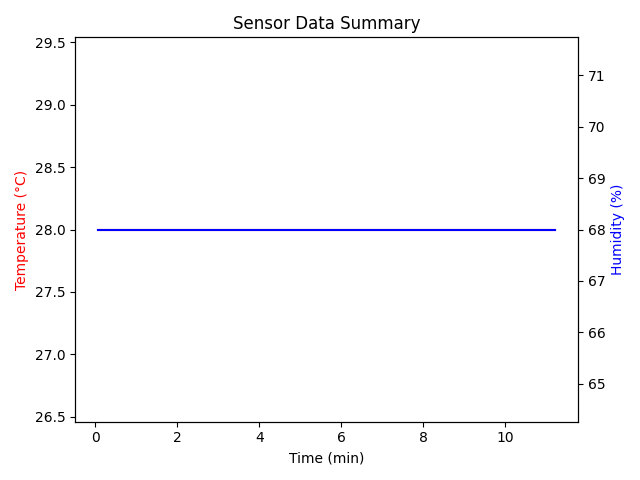
\includegraphics[width=0.6\linewidth]{10min_NormalConditions.png}
    \caption{Control test without air conditioning}
    \label{fig:enter-label}
\end{figure}
For the second plot, a fan was turned on and we noticed fluctuations in temperature and humidity, illustrating system responsiveness to environmental changes.
\begin{figure}[h!]
    \centering
    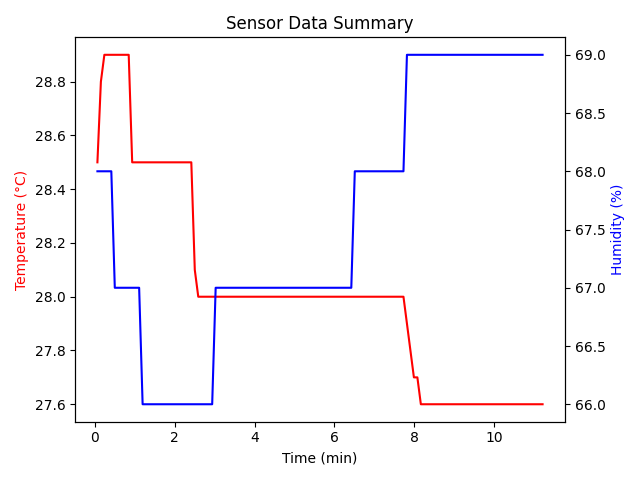
\includegraphics[width=0.6\linewidth]{10min_WithAirConditioning.png}
    \caption{Sensor data with air conditioning}
    \label{fig:enter-label}
\end{figure}
% --- End Results section with updated figure filenames ---

\newpage

\section{Future Work}

In the next activity, the system will be extended to incorporate LoRa communication to enable long-range, low-power data transmission between two ESP32 boards. One ESP32 will act as a sensor node, collecting environmental data and sending it via LoRa to a second ESP32 that functions as a gateway. This gateway will then publish the received data to the MQTT broker, preserving the architecture already developed in this activity. This setup will allow exploration of hybrid IoT communication models that combine short-range MQTT and long-range LoRa protocols, making the system suitable for remote or hard-to-access deployments.

\section{Conclusions}
This activity provided practical insight into implementing MQTT in IoT environments. MQTT's efficiency, especially its lightweight and energy-saving nature, makes it ideal for sensor-based applications. Running Mosquitto in Docker proved to be an effective method for maintaining a clean, reproducible environment. Overall, the project demonstrated the feasibility and robustness of MQTT-based communication for real-time data acquisition and visualization in IoT systems.

\end{document}
